% Created 2024-04-11 Thu 11:17
% Intended LaTeX compiler: pdflatex
\documentclass[a4paper, 11pt]{article}
\usepackage[utf8]{inputenc}
\usepackage[T1]{fontenc}
\usepackage{graphicx}
\usepackage{longtable}
\usepackage{wrapfig}
\usepackage{rotating}
\usepackage[normalem]{ulem}
\usepackage{amsmath}
\usepackage{amssymb}
\usepackage{capt-of}
\usepackage{hyperref}
\usepackage[newfloat]{minted}
\RequirePackage{listings}
\RequirePackage{fancyvrb}
\DefineVerbatimEnvironment{verbatim}{Verbatim}{fontsize=\scriptsize}
\DefineVerbatimEnvironment{lstlisting}{Verbatim}{fontsize=\scriptsize}
\renewcommand\familydefault{\sfdefault}
\usepackage{python}
\usepackage{tikz}
\usepackage{amsmath, bm}
\usepackage{arev}
\usepackage{minted}
\usemintedstyle{borland}
\author{Huiyuan Chua}
\date{\today}
\title{Examination of DDPM and CEM on Bayesian Inversion problems.}
\hypersetup{
 pdfauthor={Huiyuan Chua},
 pdftitle={Examination of DDPM and CEM on Bayesian Inversion problems.},
 pdfkeywords={},
 pdfsubject={},
 pdfcreator={Emacs 29.1 (Org mode 9.6.6)}, 
 pdflang={English}}
\begin{document}

\maketitle
\tableofcontents


\section{Problem Statement}
\label{sec:org0e26f15}
This is an investigation into the use of diffusion models to solve the problem discussed in (Adler, Jonas and Öktem, Ozan, 2018). Specifically, we use DDPM and CEM to model the problems. We want to investigate if DDPM and CEM will perform better than the reference method/model ((Adler, Jonas and Öktem, Ozan, 2018)) to denoise ultra low dose CT scans, and produce higher quality CT scans similar to the normal dose images.

In a CT scan of a subjectsbegy2pts, multiple 2D projections are generated for each angle of projection. Projections are created by the forward projection algorithm,and measures the attenutation (reduction in intensity) of the x-ray beam (cast no the subject towards the deector). A sinogram consist of mutiple projections stacked together. We can then reconstruct a 3D image of the subject of interest through a back projection algorithm such as filtered back projection (FBP). Filtered back projection is the industry standard to reconstruct images from sinograms because it is fast and robust. FBP applies a image de-blur filter (sharpen) to the projection (sinogram) and then back project the resulting projection to a 3D image. In back projection, we map the data in detector space to image space.

In (Adler, Jonas and Öktem, Ozan, 2018), we train two neural networks (GAN) to assist in the analysis of ultra low dose CT scans. An ultra low dose CT scan is simulated from a normal dose CT scan image. Projections are sampled from the normal dose image and Poisson noise is added to the projections. The ultra low dose CT image is then reconstructed using filtered back projection (FBP). The first neural network (deep posterior sampling) produces (high quality) sample images from the ultra low dose images. The second neural network (deep direct estimation) returns the mean and variance (of what the normal dose should be) given an ultra lose dose image.

(Moen, Taylor R. and Chen, Baiyu and Holmes III, David R. and Duan, Xinhui and Yu, Zhicong and Yu, Lifeng and Leng, Shuai and Fletcher, Joel G. and McCollough, Cynthia H., 2021) provides an overview of the data provided for the grand challenge. In particular, the low dose projection (DICOM-CT-PD) are simulated from the normal dose projections by adding Poisson noise.

\subsection{Filtered Back Projection (FBP)}
\label{sec:org6bd8ded}
Found a site on filtered back projection \url{https://howradiologyworks.com/filtered-backprojection-fbp-illustrated-guide-for-radiologic-technologists/\#:\~:text=Back\%20projection\%20is\%20the\%20process,Filtered\%20Backprojection\%20and\%20Iterative\%20Reconstruction}. A traditional x-ray scan gives us a 2d image of a subject of interest from a view (usually in front of the patient for a chest scan). One 2d image does not provide us a very good understanding of the subject. A forward projection algorithm instead takes multiple 2d images of a the subject from multiple and different angles/views. The end results are \uline{sinograms}. Each line/row in a sinogram corresponds to 2d image taken of the subject at particular view. A sinogram is so named because each point in the subject corresponds traces a sinusoid curve.

Given knowledge of how a forward projection works, we can reverse the process (which we call back projection) to reconstruct an image of the subject. Because the back projection (BP) is performed one view at a time, the resulting reconstructed image is a blurred image (\url{https://www.youtube.com/watch?v=YvYIkbiRMy0}). To remedy this problem, we can apply a sharpening step (or image deblurring). This image deblurring can be applied in three different manner:
\begin{enumerate}
\item BP projection to image then apply image de-blur
\item De-blur projection then BP to image
\item De-blur projection, BP to image, then finally de-blur again
\end{enumerate}
The second option (called Filtered Back Projection or FBP) is the most common as it is fast and robust. Back projection is the process of mapping the data from the detector space to the image space, while forward projection is the process of mapping the data in the image space to the detector space.

\section{Data}
\label{sec:org8cc9c92}
We use data from 2016 Low Dose CT Grand Challenge (\url{https://www.aapm.org/grandchallenge/lowdosect/\#testDatasets}). Training data is downloaded from box at \url{https://aapm.app.box.com/s/eaw4jddb53keg1bptavvvd1sf4x3pe9h}. (\url{https://www.imagewisely.org/Imaging-Modalities/Computed-Tomography/Image-Reconstruction-Techniques}) The data contains images reconstructed using two reconstruction kernels B30 and D45. Reconstruction kernels (also called “filter” or “algorithm”) affects the image quality. There is a tradeoff between spatial resolution and noise. A smoother kernel generates images with lower noise but with reduced spatial resolution. A sharper kernel generates images with higher spatial resolution, but increases the image noise. Spatial resolution in CT is the ability to differentiate objects of different density. A high spatial resolution is important to distinguish objects that are close to one another.

Patient\textsubscript{Data} directory contains the reconstructed images and projections (in DICOM-CT-PD format) of the CT scans.
Ancillary\textsubscript{Information} contains detailed documentation on the file format DICOM-CT-PD (vendor neutral DICOM format), and lesion information.

Full (normal) and associate quarter (low) dose projections (.DCM) and associated reconstructed images (.IMA) are provided by Mayo clinic. The low dose projections are simulated from the normal dose projections (McCollough, Cynthia H. and Bartley, Adam C. and Carter, Rickey E. and Chen, Baiyu and Drees, Tammy A. and Edwards, Phillip and Holmes, David R. and Huang, Alice E. and Khan, Farhana and Leng, Shuai and McMillan, Kyle L. and Michalak, Gregory J. and Nunez, Kristina M. and Yu, Lifeng and Fletcher, Joel G., 2017). The training data contain data from ten patients while the testing data contain data from twenty patients. For each patient and dosage level, there are \textasciitilde{}48k projection files and 225 reconstructed images. Each 225 reconstructed images are 2D images which forms a 3D view of the patient. Mayo has provided reconstructed images using two thickness (1mm and 3mm) and two kernels (B30 and D45). Hence, for every patient, we have a total of 2 x 2 x 2 x 225 = 1800 image files.

In the Helical scan, pitch refers to the movement of the table in the z-axis relative to the height of the detector. A helical pitch of 1.0 means the table will move a distance equal to the height of the detector resulting in scans which do not overlap and do not have gaps. A helical pitch of 0.5 means the table will move a distance equal to half the height of the detector resulting in scans that overlap. This is usually done to improve spatial resolution.

We examine some full dose samples from the training images.
\begin{minted}[]{python}
from skimage.transform import iradon
from pydicom import dcmread
import matplotlib.pyplot as plt
import numpy as np
from pathlib import Path
import tqdm

import utils

path=f'{Path.home()}/Documents/data/Mayo_Grand_Challenge/Patient_Data'

ima_path=f'{path}/Training_Image_Data/3mm B30'
ima_fd_path=f'{ima_path}/full_3mm/L067/full_3mm'

pathlist = Path(ima_fd_path).rglob('*.IMA')
ima_files = [ima for ima in pathlist]

ww = 350
wl = 50
n = 3
images=[]
ima_batch = np.random.choice(ima_files, size=n**2, replace=False)
fig, axs = plt.subplots(n, n, figsize=(3 *n, 3 * n), sharex=True, sharey=True)
_ = fig.tight_layout()
for i, ima_file in tqdm.tqdm(enumerate(ima_batch)):
    ima = dcmread(ima_file)
    image = ima.pixel_array

    # convert to HU
    hu_values = ima.RescaleSlope * image + ima.RescaleIntercept
    densities = (hu_values + 1000)/1000
    images.append(densities)
    ax = axs[i // n][i % n]
    #ax.imshow(image, cmap=plt.cm.Greys_r,)
    ax.grid(None)
    ax.imshow(utils.window_image(hu_values, ww, wl), cmap=plt.cm.Greys_r,)
plt.show()
\end{minted}

\begin{verbatim}
9it [00:00, 285.00it/s]

\end{verbatim}

\begin{center}
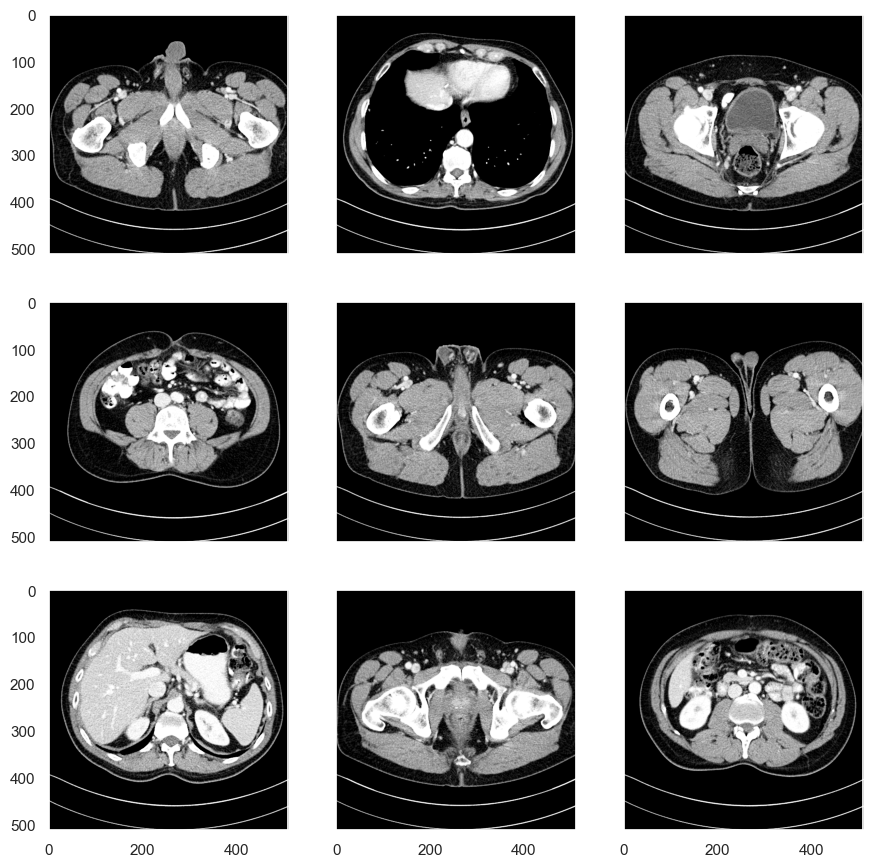
\includegraphics[width=.9\linewidth]{./.ob-jupyter/60530960a5453d2cbb849a8caa49c64bf7d7626b.png}
\end{center}

\subsection{scikit-image}
\label{sec:org595aee9}
We apply forward projection on the batch to obtain their respective sinograms (Radon transform).
\begin{minted}[,frame=single, linenos, breaklines, tabsize=2]{python}
import numpy as np
import matplotlib.pyplot as plt
from skimage.data import shepp_logan_phantom
from skimage.transform import radon, rescale
import tqdm

sinograms = []
fig, axs = plt.subplots(n, n, figsize=(3 *n, 3 * n), sharex=True, sharey=True)
_ = fig.tight_layout()
for i, image in tqdm.tqdm(enumerate(images)):
    ax = axs[i // n][i % n]

    theta = np.linspace(0., 180., max(image.shape), endpoint=False)
    sinogram = radon(image, theta=theta, circle=False)
    sinograms.append(sinogram)
    dx, dy = 0.5 * 180.0 / max(image.shape), 0.5 / sinogram.shape[0]
    ax.grid(None)
    ax.imshow(sinogram, cmap=plt.cm.Greys_r,
               extent=(-dx, 180.0 + dx, -dy, sinogram.shape[0] + dy),
               aspect='auto')

    ax.imshow(sinogram)
plt.show()
\end{minted}

\begin{verbatim}
9it [00:20,  2.24s/it]

\end{verbatim}

\begin{center}
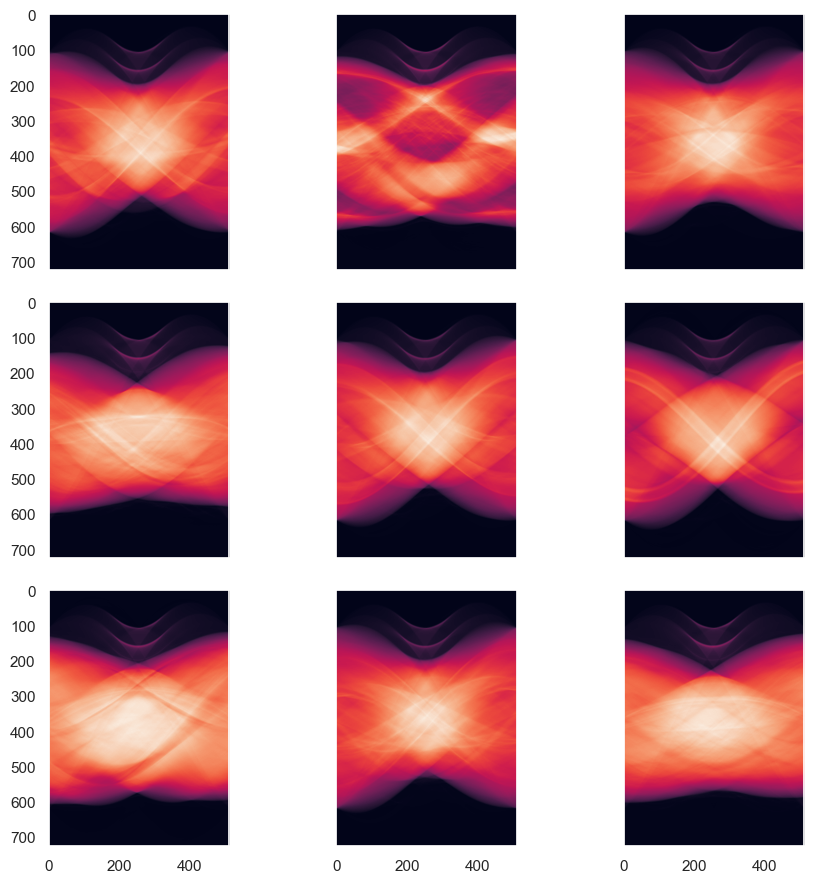
\includegraphics[width=.9\linewidth]{./.ob-jupyter/dc176021f0a9c60e509498d6f9d407a2ec448a35.png}
\end{center}

We now apply filtered back projection to reconstruct the original image using the filter "ramp".
\begin{minted}[,frame=single, linenos, breaklines, tabsize=2]{python}
from skimage.transform import iradon
from pydicom import dcmread
import matplotlib.pyplot as plt

import utils

sinogram = sinograms[4]
image = images[4] * 1000 - 1000
reconstruction_fbp = iradon(sinogram, theta=theta, filter_name='ramp', circle=False) * 1000 - 1000
error = reconstruction_fbp - image
print(f'FBP rms reconstruction error: {np.sqrt(np.mean(error**2)):.3g}')

ww = 350
wl = 50

imkwargs = dict(vmin=-0.2, vmax=0.2)
fig, (ax1, ax2, ax3) = plt.subplots(1, 3, figsize=(8, 4.5), sharex=True, sharey=True)
_ = fig.tight_layout()
ax1.set_title("Ground Truth")
ax1.grid(None)
ax1.imshow(utils.window_image(image, ww, wl), cmap=plt.cm.Greys_r)
ax2.set_title("FBP image")
ax2.grid(None)
ax2.imshow(utils.window_image(reconstruction_fbp, ww, wl), cmap=plt.cm.Greys_r)
ax3.set_title("Reconstruction error\nFiltered back projection")
ax3.grid(None)
ax3.imshow(error, cmap=plt.cm.Greys_r, **imkwargs)
plt.show()
\end{minted}

\begin{verbatim}
FBP rms reconstruction error: 10.6
\end{verbatim}

\begin{center}
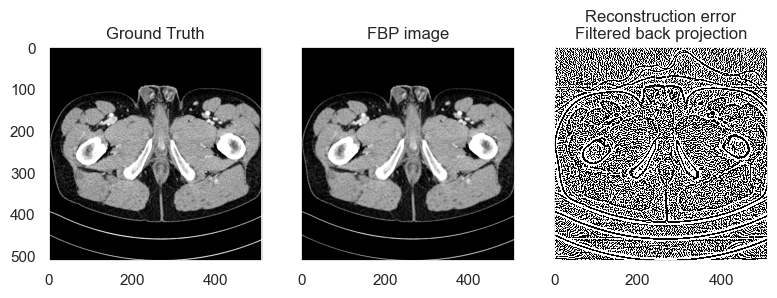
\includegraphics[width=.9\linewidth]{./.ob-jupyter/bf8b320469e40ad55860556539c903c1f6c6ffe0.png}
\end{center}

\subsection{Ultra Low Dose Simulation}
\label{sec:org6ab8f3c}
We adopt the second method of generating low dose images from normal dose images (Elhamiasl, Masoud and Nuyts, Johan, 2020). Specifically, we generate virtual projections from rescontructed full dose images, simulate noise due to a lower dosage, and reconstruct the image.
((Yi, Xin and Babyn, Paul, 2018)) \(N\sim \text{Poisson}(N_0 \exp(-y)) + \text{Gaussian}(0, \sigma_e^2)\) where \(N_0\) is the intensity of the x-ray source, \(y\) is the sinogram data, and \(\sigma_e^2\) represent the eletrical noise standard deviation.
\begin{minted}[,frame=single, linenos, breaklines, tabsize=2]{python}
import numpy as np

N0 = 100000 # x-ray influx
slice_thickness = 0.03 # in cm
epsilon = 5 # small number > 0 that reflects smallest possible detected photon count
sinogramCT = N0 * np.exp(-sinogram * slice_thickness)
sinogram_noisy = np.random.poisson(sinogramCT) # poissrnd(sinogram)
sinogram_out = -np.log(sinogram_noisy/N0)/slice_thickness

idx = np.isinf(sinogram_out)
sinogram_out[idx] = -np.log(epsilon/N0)/slice_thickness
# we need to update infinity values to -log(epsilon/N0)/0.0625 where epsilon =5

reconstruction_fbp = iradon(sinogram_out, theta=theta, filter_name='ramp') * 1000 - 1000

#plt.imshow(sinogram_out)
plt.imshow(utils.window_image(reconstruction_fbp, ww, wl), cmap=plt.cm.Greys_r)
\end{minted}

\begin{verbatim}
/var/folders/bc/r2l4k0lx343ds2rjs_2mjns00000gn/T/ipykernel_1478/3904578395.py:8: RuntimeWarning: divide by zero encountered in log
  sinogram_out = -np.log(sinogram_noisy/N0)/slice_thickness
<matplotlib.image.AxesImage at 0x1764d8ed0>
\end{verbatim}

\begin{center}
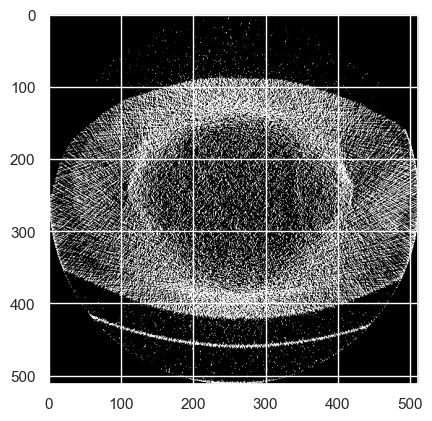
\includegraphics[width=.9\linewidth]{./.ob-jupyter/a2c5cd91c793b7ab083a82fbbf06731021691179.png}
\end{center}

For simplicity, let's add Poisson noise directly to the full dose image.
\begin{minted}[,frame=single, linenos, breaklines, tabsize=2]{python}
import numpy as np
import utils
PEAK = 1.
image_in = utils.window_image(image, ww, wl)
noise_mask = np.random.poisson(image_in/255. * PEAK)/ PEAK * 255.
image_noisy = np.clip(image_in + noise_mask, 0., 255.)
plt.imshow(image_noisy, cmap=plt.cm.Greys_r)
\end{minted}

\begin{verbatim}
<matplotlib.image.AxesImage at 0x1505d5190>
\end{verbatim}

\begin{center}
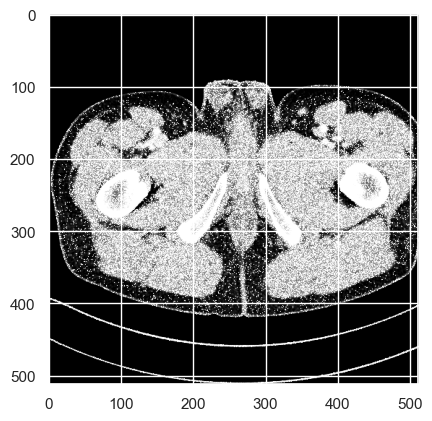
\includegraphics[width=.9\linewidth]{./.ob-jupyter/867b134dcccbb5541e76d3d5c51efc23c8aac807.png}
\end{center}

\subsection{Preprocessing data for training}
\label{sec:org12845e9}
Here, we retrieve Mayo training data in pairs (full dose, quarter dose), and compare a few samples.
\begin{minted}[,frame=single, linenos, breaklines, tabsize=2]{python}
import mayo
import numpy as np
import matplotlib.pyplot as plt

import utils

path=f'{Path.home()}/Documents/data/Mayo_Grand_Challenge/Patient_Data/Training_Image_Data/3mm B30'
training_data = mayo.get_training_data(path, 112, 113) # pull the middle slices of each patient
fd_ima, qd_ima = training_data[len(training_data) // 2]
noise = fd_ima - qd_ima

print(f'noise: {np.sqrt(np.mean(noise**2)):.3g}')

imkwargs = dict(vmin=-0.2, vmax=0.2)
fig, (ax1, ax2, ax3) = plt.subplots(1, 3, figsize=(8, 4.5), sharex=True, sharey=True)
_ = fig.tight_layout()
_ = ax1.set_title("full dose image")
_ = ax1.imshow(utils.normalize_image(fd_ima), cmap=plt.cm.Greys_r)
_ = ax2.set_title("quarter dose image")
_ = ax2.imshow(utils.normalize_image(qd_ima), cmap=plt.cm.Greys_r)
_ = ax3.set_title("noise")
_ = ax3.imshow(noise, cmap=plt.cm.Greys_r, **imkwargs)
plt.show()

\end{minted}

\begin{verbatim}
loading patient data: 100% 10/10 [00:00<00:00, 65.98it/s]

noise: 0.00468
\end{verbatim}

\begin{center}
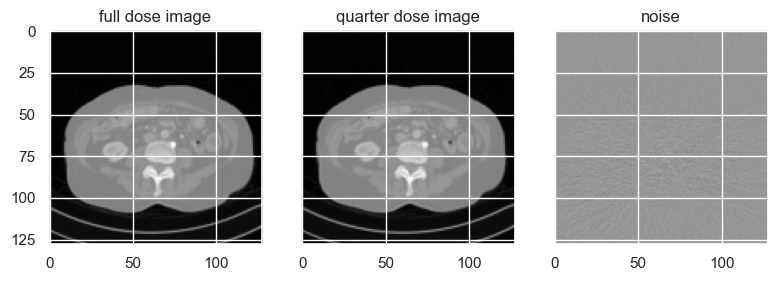
\includegraphics[width=.9\linewidth]{./.ob-jupyter/87b4f042c9bbc291a64110740ae09645af97d617.png}
\end{center}
We preprocess the data to 128x128x1 and window to a range of 350 HU and centered about 50 HU. Importantly, the data is saved in HDF5 format. This allows us to not load the entire training or test data into memory and use the data in a similar fashion to numpy arrays.
\begin{minted}[,frame=single, linenos, breaklines, tabsize=2]{python}
import h5py
from pathlib import Path
import matplotlib.pyplot as plt

import mayo
import utils

path=f'{Path.home()}/Documents/data/Mayo_Grand_Challenge/Patient_Data/Training_Image_Data/3mm B30'
training_data = mayo.get_training_data(path)
test_data = mayo.get_test_data(path)

with h5py.File(f'{Path.home()}/Documents/data/mayo.hdf5', 'w') as hf:

  train = hf.create_dataset('train', data=training_data, compression="gzip", chunks=True)
  test = hf.create_dataset('test', data=test_data, compression="gzip", chunks=True)
  fd_data, ld_data, uld_data = test[36]

ww = 350
wl = 50

fd_data = fd_data * ww - wl
ld_data = ld_data * ww - wl
uld_data = uld_data * ww - wl

fig, (ax1, ax2, ax3) = plt.subplots(1, 3, figsize=(8, 4.5), sharex=True, sharey=True)
figures = [('Ground Truth', ax1, utils.window_image(fd_data, ww, wl)),
           ('Low Dose Image', ax2, utils.window_image(ld_data, ww, wl)),
           ('Ultra Low Dose Image', ax3, utils.window_image(uld_data, ww, wl))]

_ = fig.tight_layout()
for title, ax, figure in figures:
  ax.grid(None)
  ax.set_title(title)
  ax.imshow(figure, cmap=plt.cm.Greys_r)

plt.show()
\end{minted}

\begin{verbatim}
loading patient data: 100% 9/9 [02:09<00:00, 14.34s/it]

loading patient data: 100% 1/1 [00:14<00:00, 14.77s/it]

\end{verbatim}

\begin{center}
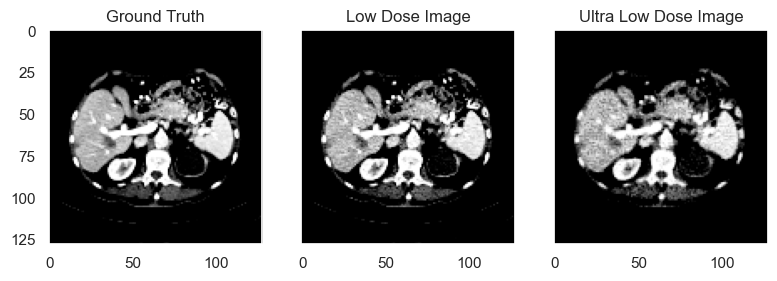
\includegraphics[width=.9\linewidth]{./.ob-jupyter/9dad22006e92686768aeab3338ada870ec4f2d9c.png}
\end{center}

\subsection{ODL examples}
\label{sec:org8cb164e}
Next, we explore if we can reconstruct images from Mayo's full dose projections (Helical scans), and how it compares with the provided images reconstructed using commercial software (weighted FBP).
\begin{minted}[,frame=single, linenos, breaklines, tabsize=2]{python}
#from pydicom import dcmread
import matplotlib.pyplot as plt
import numpy as np
from pathlib import Path

home_path = str(Path.home())
path=home_path + '/Documents/data/Mayo_Grand_Challenge/Patient_Data'

dcm_path=path + '/Training_Projection_Data/L067'
dcm_fd_path=dcm_path + '/DICOM-CT-PD_FD'

import odl
from odl.contrib.datasets.ct import mayo

mayo_dir = home_path + '/Documents/data/Mayo_Grand_Challenge/Patient_Data'  # replace with your local folder

# Load reference reconstruction
#volume_folder = mayo_dir + '/Training Cases/L067/full_1mm_sharp'
volume_folder = mayo_dir + '/Training_Image_Data/3mm B30/full_3mm/L067/full_3mm'
partition, volume = mayo.load_reconstruction(volume_folder)

# Load a subset of the projection data
#data_folder = mayo_dir + '/Training Cases/L067/full_DICOM-CT-PD'
data_folder = mayo_dir + '/Training_Projection_Data/L067/DICOM-CT-PD_FD'
geometry, proj_data = mayo.load_projections(data_folder,
                                          indices=slice(20000, 28000))

# Reconstruction space and ray transform
space = odl.uniform_discr_frompartition(partition, dtype='float32')
ray_trafo = odl.tomo.RayTransform(space, geometry)

# Define FBP operator
fbp = odl.tomo.fbp_op(ray_trafo, padding=True)

# Tam-Danielsson window to handle redundant data
td_window = odl.tomo.tam_danielson_window(ray_trafo, n_pi=3)

# Calculate FBP reconstruction
fbp_result = fbp(td_window * proj_data)

# Compare the computed recon to reference reconstruction (coronal slice)
ref = space.element(volume)
fbp_result.show('Recon (coronal)', clim=[0.7, 1.3])
ref.show('Reference (coronal)', clim=[0.7, 1.3])
(ref - fbp_result).show('Diff (coronal)', clim=[-0.1, 0.1])

# Also visualize sagittal slice (note that we only used a subset)
coords = [0, None, None]
fbp_result.show('Recon (sagittal)', clim=[0.7, 1.3], coords=coords)
ref.show('Reference (sagittal)', clim=[0.7, 1.3], coords=coords)
(ref - fbp_result).show('Diff (sagittal)', clim=[-0.1, 0.1], coords=coords)

#n = 3
#sinograms=[]
#sinogram_batch = np.random.choice(dcm_files, size=n**2, replace=False)
#fig, axs = plt.subplots(n, n, figsize=(3 *n, 3 * n), sharex=True, sharey=True)
#_ = fig.tight_layout()
#for i, sinogram_file in enumerate(sinogram_batch):
#    dcm = dcmread(sinogram_file)
#    sinogram = dcm.pixel_array
#    sinograms.append(sinogram)
#    ax = axs[i // n][i % n]
#    ax.imshow(sinogram, cmap=plt.cm.Greys_r,)
#plt.show()
\end{minted}

\begin{verbatim}
loading volume data: 100%|██████████| 223/223 [00:02<00:00, 75.90it/s]
Loading projection data:   0%|          | 0/8000 [00:00<?, ?it/s]
\end{verbatim}

\begin{verbatim}

AttributeErrorTraceback (most recent call last)
<ipython-input-9-8dc0f17f65e8> in <module>()
     24 data_folder = mayo_dir + '/Training_Projection_Data/L067/DICOM-CT-PD_FD'
     25 geometry, proj_data = mayo.load_projections(data_folder,
---> 26                                           indices=slice(20000, 28000))
     27 
     28 # Reconstruction space and ray transform

~/miniconda3/envs/odlenv/lib/python3.5/site-packages/odl/contrib/datasets/ct/mayo.py in load_projections(folder, indices)
    102         coefficient (g/cm^3). Its unit is thus g/cm^2.
    103     """
--> 104     datasets, data_array = _read_projections(folder, indices)
    105 
    106     # Get the angles

~/miniconda3/envs/odlenv/lib/python3.5/site-packages/odl/contrib/datasets/ct/mayo.py in _read_projections(folder, indices)
     57         rows = dataset.NumberofDetectorRows
     58         cols = dataset.NumberofDetectorColumns
---> 59         hu_factor = dataset.HUCalibrationFactor
     60         rescale_intercept = dataset.RescaleIntercept
     61         rescale_slope = dataset.RescaleSlope

~/miniconda3/envs/odlenv/lib/python3.5/site-packages/dicom/dataset.py in __getattr__(self, name)
    255         if tag not in self:
    256             raise AttributeError("Dataset does not have attribute "
--> 257                                  "'{0:s}'.".format(name))
    258         else:  # do have that dicom data_element
    259             return self[tag].value

AttributeError: Dataset does not have attribute 'HUCalibrationFactor'.
\end{verbatim}

\section{DDPM}
\label{sec:orgcf0b9af}
DDPM specific parameters.
\begin{minted}[,frame=single, linenos, breaklines, tabsize=2]{python}
import os

SEED=42
MIN_BETA, MAX_BETA = 1e-4, 0.02
K = 200
N_EPOCH = 30
BATCH_SIZE = 10
PROJECT_DIR=os.path.abspath('.')
\end{minted}

\subsection{Training}
\label{sec:org7f3233a}
First, let's make sure we have the correct shapes for training data inputs and predictions.
\begin{minted}[,frame=single, linenos, breaklines, tabsize=2]{python}
from jax import random
import jax.numpy as jnp
import numpy as np
from pathlib import Path

import utils
import mayo

key = random.PRNGKey(42)
state = utils.create_training_state(key=key)
path=f'{Path.home()}/Documents/data/Mayo_Grand_Challenge/Patient_Data/Training_Image_Data/3mm B30'
training_data = mayo.get_training_data(path, 112, 113)

x_0_fd = training_data[:, 0]
x_0_ld = training_data[:, 1]
x_k = jnp.concatenate((x_0_fd, x_0_ld), axis=-1)
n = training_data.shape[0]
k = random.choice(key, np.arange(200), shape=(n,))
predictions = state.apply_fn(state.params, x_k, k)
print(f'training input shape (x_t, t): {x_k.shape}, {k.shape}')
print(f'predictions shape (x_0): {predictions.shape}')
\end{minted}

\begin{verbatim}
loading patient data: 100% 10/10 [00:00<00:00, 76.08it/s]

training input shape (x_t, t): (10, 128, 128, 2) {(10,)}
predictions shape (x_0): (10, 128, 128, 1)
\end{verbatim}

Training is performed via a python script \url{train\_ddpm.py}. We examine the average epoch loss with the following code:
\begin{minted}[,frame=single, linenos, breaklines, tabsize=2]{python}
import pandas as pd
import matplotlib.pyplot as plt
import seaborn as sns
import os

import utils

PROJECT_DIR=os.path.abspath('.')
ddpm_loss_log = utils.load_loss_log(f'{PROJECT_DIR}/ddpm_loss_log.npy')

# plot losses
df = pd.DataFrame([(int(x), float(y)) for x, _, y in ddpm_loss_log], columns=['epoch', 'loss'])
sns.relplot(df, x='epoch', y='loss', kind='line')

_ = plt.tight_layout()
_ = plt.show()
\end{minted}

\begin{center}
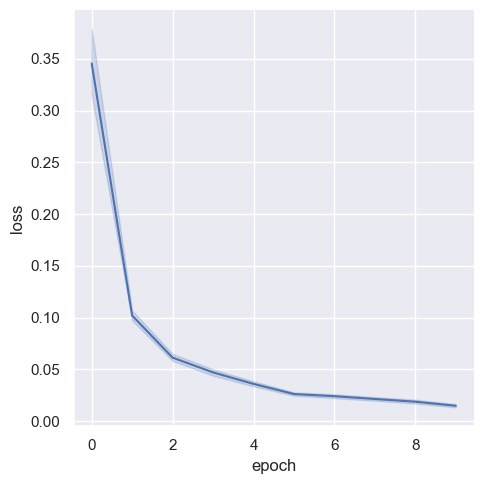
\includegraphics[width=.9\linewidth]{./.ob-jupyter/98b946f3ee6dbe5becc443cc009687eff61363d4.png}
\end{center}

\subsection{Sampling}
\label{sec:org385c625}
We sample images from the trained DDPM model.
\begin{minted}[,frame=single, linenos, breaklines, tabsize=2]{python}
import matplotlib.pyplot as plt
import optax
from jax import random
import jax.numpy as jnp
from tqdm import tqdm
import numpy as np

import utils
import mayo

def sample(state, condition, n, betas, key):
  # random white noise X_T
  key, subkey = random.split(key)
  x_k = random.normal(subkey, shape=(n, condition.shape[0], condition.shape[1], 1))

  #dts = np.array([ts[i] - ts[i-1] for i in range(1, steps+1)])
  #betas = 1- np.exp(-dts)
  alphas = 1 - betas
  alpha_bars = jnp.cumprod(alphas)
  #alpha_bars = jnp.array([alphas[:i+1].prod() for i in range(len(alphas))]) # workaround for metal problem with jnp.cumprod

  condition = np.repeat(condition.reshape((1, condition.shape[0], condition.shape[1], 1)), n, axis=0)

  # sample in reverse from T=10 to 0.0 in evenly distributed steps
  #for i in tqdm(range(steps)[::-1]):
  for k in range(len(betas))[::-1]:
    alpha = alphas[k]
    beta = betas[k]
    alpha_bar_k = alpha_bars[k]

    key, subkey = random.split(key)
    z = jnp.where(k > 1, random.normal(subkey, shape=x_k.shape), jnp.zeros_like(x_k))
    sigma_k = jnp.sqrt(beta) # option 1; see DDPM 3.2
    #sigma_k = jnp.sqrt((1-alpha_bars[k-1])/(1 - alpha_bar_k) * beta) # option 2; see DDPM 3.2

    inputs = jnp.concatenate((x_k, condition), axis=-1)

    x_k = 1/jnp.sqrt(alpha) * (x_k - beta/jnp.sqrt(1 - alpha_bar_k) * state.apply_fn(state.params, inputs, k * jnp.ones((x_k.shape[0], )))) + sigma_k * z

    #x_k = jnp.clip(x_k, -1., 1.) # should we clip ...
    x_t = jnp.clip(x_t, -3., 3.)
    #x_t = normalize_to_neg_one_to_one(x_t) # or scale?

  return x_k

key = random.PRNGKey(SEED)

# use the best params
file_path, epoch, step, loss = utils.find_latest_pytree(f'{PROJECT_DIR}/ddpm_params_*.npy')
ddpm_state = utils.create_training_state(params_file=f'{PROJECT_DIR}/ddpm_params_{epoch}_{step}_{loss}.npy')
print(f'using parameters from epoch {epoch} with loss {loss}')

betas = jnp.linspace(MIN_BETA, MAX_BETA, K)
path=f'{Path.home()}/Documents/data/Mayo_Grand_Challenge/Patient_Data/Training_Image_Data/3mm B30'
training_data = mayo.get_training_data(path, 112, 113)
n = (len(training_data) // 10) * 9
test_data = training_data[n:]
test_data = []
n_samples = 1000

fd_data, ld_data = training_data[0]
result = np.zeros(fd_data.shape)

for i in tqdm(range(n_samples // BATCH_SIZE)):
  # generate x_0 from noise
  key, subkey = random.split(key)
  x_0_tilde = sample(ddpm_state, ld_data, BATCH_SIZE, betas, subkey)

  result = result + np.sum(x_0_tilde, axis=0)

result = result / n_samples
error = fd_data - result
print(f'error: {np.mean(error)}')

# plot and compare last sample
imkwargs = dict(vmin=-0.2, vmax=0.2)
fig, axs = plt.subplots(2, 2, figsize=(8, 4.5), sharex=True, sharey=True)
_ = fig.tight_layout()
_ = axs[0, 0].set_title("full dose image")
_ = axs[0, 0].imshow(utils.normalize_image_to_greyscale(fd_data), cmap=plt.cm.Greys_r)
_ = axs[0, 1].set_title("quarter dose image")
_ = axs[0, 1].imshow(utils.normalize_image_to_greyscale(ld_data), cmap=plt.cm.Greys_r)
_ = axs[1, 0].set_title("DDPM")
_ = axs[1, 0].imshow(utils.normalize_image_to_greyscale(result), cmap=plt.cm.Greys_r)
_ = axs[1, 1].set_title("error")
_ = axs[1, 1].imshow(error, cmap=plt.cm.Greys_r, **imkwargs)

plt.show()
\end{minted}

\begin{verbatim}
  Platform 'METAL' is experimental and not all JAX functionality may be correctly supported!
  2024-03-23 12:48:02.264962: W pjrt_plugin/src/mps_client.cc:563] WARNING: JAX Apple GPU support is experimental and not all JAX functionality is correctly supported!
  Metal device set to: Apple M1
  using parameters from epoch 22 with loss 0.00825
  loading patient data: 100% 10/10 [00:00<00:00, 59.47it/s]

  100% 200/200 [03:55<00:00,  1.18s/it]

  100% 200/200 [03:50<00:00,  1.15s/it]
100% 200/200 [03:49<00:00,  1.15s/it]
100% 200/200 [03:48<00:00,  1.14s/it]
100% 200/200 [03:48<00:00,  1.14s/it]
100% 200/200 [03:48<00:00,  1.14s/it]
100% 200/200 [03:50<00:00,  1.15s/it]
100% 200/200 [03:49<00:00,  1.15s/it]
100% 200/200 [03:49<00:00,  1.15s/it]
100% 200/200 [03:49<00:00,  1.15s/it]
100% 200/200 [03:48<00:00,  1.14s/it]
100% 200/200 [03:48<00:00,  1.14s/it]
100% 200/200 [03:48<00:00,  1.14s/it]
100% 200/200 [03:48<00:00,  1.14s/it]
100% 200/200 [03:48<00:00,  1.14s/it]
100% 200/200 [03:48<00:00,  1.14s/it]
100% 200/200 [03:54<00:00,  1.17s/it]
100% 200/200 [03:48<00:00,  1.14s/it]
100% 200/200 [03:48<00:00,  1.14s/it]
100% 200/200 [03:48<00:00,  1.14s/it]
100% 200/200 [03:49<00:00,  1.15s/it]
100% 200/200 [03:48<00:00,  1.14s/it]
100% 200/200 [03:48<00:00,  1.14s/it]
100% 200/200 [03:48<00:00,  1.14s/it]
100% 200/200 [03:51<00:00,  1.16s/it]
100% 200/200 [03:48<00:00,  1.14s/it]
100% 200/200 [03:49<00:00,  1.15s/it]
100% 200/200 [03:48<00:00,  1.14s/it]
100% 200/200 [03:48<00:00,  1.14s/it]
100% 200/200 [03:52<00:00,  1.16s/it]
100% 200/200 [03:50<00:00,  1.15s/it]
100% 200/200 [03:52<00:00,  1.16s/it]
100% 200/200 [03:51<00:00,  1.16s/it]
100% 200/200 [03:49<00:00,  1.15s/it]
100% 200/200 [03:49<00:00,  1.15s/it]
100% 200/200 [03:49<00:00,  1.15s/it]
100% 200/200 [03:49<00:00,  1.15s/it]
100% 200/200 [03:48<00:00,  1.14s/it]
100% 200/200 [03:49<00:00,  1.15s/it]
100% 200/200 [03:51<00:00,  1.16s/it]
100% 200/200 [03:49<00:00,  1.15s/it]
100% 200/200 [03:48<00:00,  1.14s/it]
100% 200/200 [03:49<00:00,  1.15s/it]
100% 200/200 [03:48<00:00,  1.14s/it]
100% 200/200 [03:49<00:00,  1.15s/it]
100% 200/200 [03:49<00:00,  1.15s/it]
100% 200/200 [03:49<00:00,  1.15s/it]
100% 200/200 [03:52<00:00,  1.16s/it]
100% 200/200 [03:49<00:00,  1.15s/it]
100% 200/200 [03:49<00:00,  1.15s/it]
100% 200/200 [03:49<00:00,  1.15s/it]
100% 200/200 [03:49<00:00,  1.15s/it]
100% 200/200 [03:49<00:00,  1.15s/it]
100% 200/200 [03:49<00:00,  1.15s/it]
100% 200/200 [03:49<00:00,  1.15s/it]
100% 200/200 [03:52<00:00,  1.16s/it]
100% 200/200 [03:49<00:00,  1.15s/it]
100% 200/200 [03:49<00:00,  1.15s/it]
100% 200/200 [03:49<00:00,  1.15s/it]
100% 200/200 [03:49<00:00,  1.15s/it]
100% 200/200 [03:49<00:00,  1.15s/it]
100% 200/200 [03:49<00:00,  1.15s/it]
100% 200/200 [03:50<00:00,  1.15s/it]
100% 200/200 [03:53<00:00,  1.17s/it]
100% 200/200 [03:49<00:00,  1.15s/it]
100% 200/200 [03:49<00:00,  1.15s/it]
100% 200/200 [03:49<00:00,  1.15s/it]
100% 200/200 [03:49<00:00,  1.15s/it]
100% 200/200 [03:49<00:00,  1.15s/it]
100% 200/200 [03:49<00:00,  1.15s/it]
100% 200/200 [03:49<00:00,  1.15s/it]
100% 200/200 [03:52<00:00,  1.16s/it]
100% 200/200 [03:49<00:00,  1.15s/it]
100% 200/200 [03:49<00:00,  1.15s/it]
100% 200/200 [03:49<00:00,  1.15s/it]
100% 200/200 [03:49<00:00,  1.15s/it]
100% 200/200 [03:49<00:00,  1.15s/it]
100% 200/200 [03:49<00:00,  1.15s/it]
100% 200/200 [03:52<00:00,  1.16s/it]
100% 200/200 [03:50<00:00,  1.15s/it]
100% 200/200 [03:49<00:00,  1.15s/it]
100% 200/200 [03:50<00:00,  1.15s/it]
100% 200/200 [03:49<00:00,  1.15s/it]
100% 200/200 [03:49<00:00,  1.15s/it]
100% 200/200 [03:49<00:00,  1.15s/it]
100% 200/200 [03:50<00:00,  1.15s/it]
100% 200/200 [03:52<00:00,  1.16s/it]
100% 200/200 [03:49<00:00,  1.15s/it]
100% 200/200 [03:49<00:00,  1.15s/it]
100% 200/200 [03:49<00:00,  1.15s/it]
100% 200/200 [03:49<00:00,  1.15s/it]
100% 200/200 [03:49<00:00,  1.15s/it]
100% 200/200 [03:49<00:00,  1.15s/it]
100% 200/200 [03:50<00:00,  1.15s/it]
100% 200/200 [03:52<00:00,  1.16s/it]
100% 200/200 [03:50<00:00,  1.15s/it]
100% 200/200 [03:50<00:00,  1.15s/it]
100% 200/200 [03:50<00:00,  1.15s/it]
100% 200/200 [03:50<00:00,  1.15s/it]
100% 200/200 [03:50<00:00,  1.15s/it]
  error: 0.11948700249195099
\end{verbatim}
\begin{center}
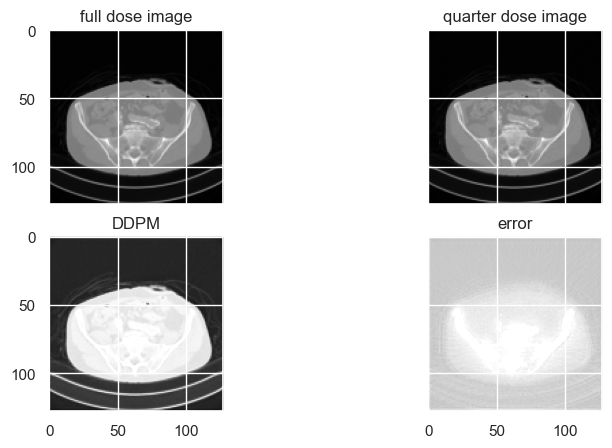
\includegraphics[width=.9\linewidth]{./.ob-jupyter/da8b230284e5503497e7e30a76f4e73bb3cc5842.png}
\end{center}

We show the results from samples generated externally.
\begin{minted}[,frame=single, linenos, breaklines, tabsize=2]{python}
import h5py
from pathlib import Path
import matplotlib.pyplot as plt

with h5py.File(f'{Path.home()}/Documents/data/mayo.hdf5', 'r') as hf:
  fd_data, ld_data = hf['test'][36]

with h5py.File(f'{Path.home()}/Documents/data/ddpm_samples.hdf5', 'r') as hf:
  samples = hf['samples']
  sample_mean = np.mean(samples, axis=0)
  sample_variance = np.var(samples, axis=0)

# plot the data
imkwargs = dict(vmin=-0.2, vmax=0.2)
fig, axs = plt.subplots(2, 2, figsize=(8, 4.5), sharex=True, sharey=True)
_ = fig.tight_layout()
_ = axs[0, 0].set_title("full dose image")
_ = axs[0, 0].imshow(utils.normalize_to_greyscale(fd_data), cmap=plt.cm.Greys_r)
_ = axs[0, 1].set_title("quarter dose image")
_ = axs[0, 1].imshow(utils.normalize_to_greyscale(ld_data), cmap=plt.cm.Greys_r)
_ = axs[1, 0].set_title("CEM mean")
_ = axs[1, 0].imshow(utils.normalize_to_greyscale(sample_mean), cmap=plt.cm.Greys_r)
_ = axs[1, 1].set_title("CEM variance")
#_ = axs[1, 1].imshow(wd(sample_variance), **imkwargs)
_ = axs[1, 1].imshow(utils.normalize_to_greyscale(sample_variance))

plt.show()
\end{minted}

\section{CEM}
\label{sec:org3ff1db7}
\begin{minted}[,frame=single, linenos, breaklines, tabsize=2]{python}
import os

SEED=42
T=10.
K=1000
BATCH_SIZE = 10
PROJECT_DIR=os.path.abspath('.')
\end{minted}
\subsection{Training}
\label{sec:org248b1ae}
Training is performed via a python script \url{train\_cem.py}. We examine the average epoch loss with the following code:
\begin{minted}[,frame=single, linenos, breaklines, tabsize=2]{python}
import pandas as pd
import matplotlib.pyplot as plt
import seaborn as sns

import utils

cem_loss_log = utils.load_loss_log(f'{PROJECT_DIR}/cem_loss_log.npy')

# plot losses
df = pd.DataFrame([(int(x), float(y)) for x, _, y in cem_loss_log], columns=['epoch', 'loss'])
sns.relplot(df, x='epoch', y='loss', kind='line')

_ = plt.tight_layout()
_ = plt.show()
\end{minted}

\begin{verbatim}
/Users/huiyuanchua/miniconda3/envs/mlenv-metal/lib/python3.11/site-packages/seaborn/_oldcore.py:1119: FutureWarning: use_inf_as_na option is deprecated and will be removed in a future version. Convert inf values to NaN before operating instead.
  with pd.option_context('mode.use_inf_as_na', True):
/Users/huiyuanchua/miniconda3/envs/mlenv-metal/lib/python3.11/site-packages/seaborn/_oldcore.py:1119: FutureWarning: use_inf_as_na option is deprecated and will be removed in a future version. Convert inf values to NaN before operating instead.
  with pd.option_context('mode.use_inf_as_na', True):
\end{verbatim}

\begin{center}
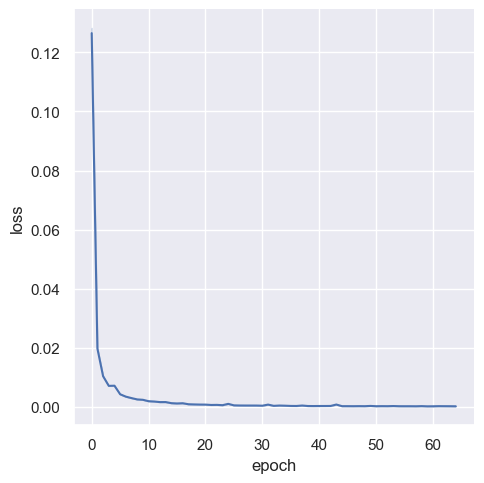
\includegraphics[width=.9\linewidth]{./.ob-jupyter/9116398acd8b24680bfcc5c9c8c5b48242340955.png}
\end{center}

\subsection{Sampling}
\label{sec:org9203451}
We sample images from the trained CEM model.
\begin{minted}[,frame=single, linenos, breaklines, tabsize=2]{python}
import matplotlib.pyplot as plt
import optax
from jax import random
import jax.numpy as jnp
from tqdm import tqdm
import numpy as np
import h5py
from pathlib import Path


import utils
from unet import Unet
import mayo

def sample(state, condition, n, ts, key):
    # random white noise X_T
    key, subkey = random.split(key)
    x_t = random.normal(subkey, shape=(n, condition.shape[0], condition.shape[1], 1))

    condition = np.repeat(condition.reshape((1, condition.shape[0], condition.shape[1], 1)), n, axis=0)

    step=0

    for k in range(len(ts))[::-1]:
      key, subkey = random.split(key)
      z = random.normal(subkey, shape=x_t.shape)

      t = ts[k]
      dt = jnp.where(k > 0, t - ts[k-1], 0.)

      inputs = jnp.concatenate((x_t, condition), axis=-1)


      f_theta = state.apply_fn(state.params, inputs, t * jnp.ones((n,)))

      # equation (40)
      s_theta = jnp.where(k > 0, x_t/(1-jnp.exp(-t))  - jnp.exp(-t/2)/(1-jnp.exp(-t)) * f_theta,  0.)

      # equation (24)
      x_t_bar = x_t - dt * s_theta
      x_t = jnp.exp(dt/2) * x_t_bar + jnp.sqrt(1-jnp.exp(-dt)) * z

      x_t = jnp.clip(x_t, -1., 1.) # should we clip ...
      #x_t = normalize_to_neg_one_to_one(x_t) # or scale?

      step=step+1

    return x_t

  key = random.PRNGKey(SEED)
  n_samples = 1000

  # use the best params
  file_path, epoch, step, loss = utils.find_latest_pytree(f'{PROJECT_DIR}/cem_params_*.npy')
  cem_state = utils.create_training_state(params_file=file_path)
  print(f'using parameters from epoch {epoch} with loss {loss}')
  ts = utils.exponential_time_schedule(T, K)
  path=f'{Path.home()}/Documents/data/Mayo_Grand_Challenge/Patient_Data/Training_Image_Data/3mm B30'

with h5py.File(f'{Path.home()}/Documents/data/mayo.hdf5', 'r') as hf:
  test_data = hf['test'][36]
  fd_data, ld_data = test_data

# create empty samples HDF5 to store samples
samples_path = f'{Path.home()}/Documents/data/cem_samples.hdf5'
with h5py.File(samples_path, 'w') as hf:
  samples = hf.create_dataset('samples', data=np.zeros((n_samples, 512, 512, 1)), compression='gzip', chunks=True)

for i in tqdm(range(n_samples // BATCH_SIZE)):
  # generate x_0 from noise
  key, subkey = random.split(key)
  x_0_tilde = sample(cem_state, ld_data, BATCH_SIZE, ts, subkey)

  # rescale in HU
  x_0_tilde = x_0_tilde * ww/2 + wl

  with h5py.File(samples_path, 'a') as hf:
    hf['samples'][(i * BATCH_SIZE):((i + 1) * BATCH_SIZE)] = x_0_tilde

with h5py.File(samples_path, 'r') as hf:
  samples = hf['samples']
  sample_mean = np.mean(samples, axis=0)
  sample_variance = np.var(samples, axis=0)

# plot the data
imkwargs = dict(vmin=-0.2, vmax=0.2)
fig, axs = plt.subplots(2, 2, figsize=(8, 4.5), sharex=True, sharey=True)
_ = fig.tight_layout()
_ = axs[0, 0].set_title("full dose image")
_ = axs[0, 0].imshow(utils.normalize_to_greyscale(fd_data), cmap=plt.cm.Greys_r)
_ = axs[0, 1].set_title("quarter dose image")
_ = axs[0, 1].imshow(utils.normalize_to_greyscale(ld_data), cmap=plt.cm.Greys_r)
_ = axs[1, 0].set_title("CEM mean")
_ = axs[1, 0].imshow(utils.normalize_to_greyscale(sample_mean), cmap=plt.cm.Greys_r)
_ = axs[1, 1].set_title("CEM variance")
#_ = axs[1, 1].imshow(wd(sample_variance), **imkwargs)
_ = axs[1, 1].imshow(utils.normalize_to_greyscale(sample_variance))

plt.show()
\end{minted}

\begin{minted}[,frame=single, linenos, breaklines, tabsize=2]{python}
import utils
import h5py
from pathlib import Path
import numpy as np
import matplotlib.pyplot as plt
from matplotlib.patches import Circle
from scipy import stats

ww = 350
wl = 50

with h5py.File(f'{Path.home()}/Documents/data/mayo.hdf5', 'r') as hf:
  fd_data, ld_data, uld_data = hf['test'][36]

fd_data = fd_data * ww - wl
ld_data = ld_data * ww - wl
uld_data = uld_data * ww - wl

samples_path=f'{Path.home()}/Documents/bayesian-inversion/cem_samples.hdf5'

with h5py.File(samples_path, 'r') as hf:

  samples = hf['samples']
  sample_mean = np.mean(samples, axis=0) * ww - wl
  sample_variance = np.var(samples, axis=0) * ww - wl
  lesion_contrast_sum = 0.
  for sample in samples:
    sample_hu = sample * ww - wl
    reference_roi = utils.get_image_region(sample_hu, reference_center, reference_radius)
    lesion_roi = utils.get_image_region(sample_hu, lesion_center, lesion_radius)
    lesion_contrast = lesion_roi.mean() - reference_roi.mean()
    lesion_contrast_sum = lesion_contrast + lesion_contrast_sum
  print(f'mean of CEM individual sample contrast = {lesion_contrast_sum/len(samples)}')

# save images for analysis
for file_name, image_data in [('full_dose.png', fd_data), ('ultra_low_dose.png', uld_data), ('cem_sample_mean.png', sample_mean)]:
  plt.clf()
  plt.imshow(utils.window_image(image_data, ww, wl), cmap=plt.cm.Greys_r)
  plt.grid(None)
  plt.savefig(file_name)

plt.clf()
# plot the data
imkwargs = dict(vmin=-0.2, vmax=0.2)
fig, axs = plt.subplots(2, 2, figsize=(8, 4.5), sharex=True, sharey=True)
_ = fig.tight_layout()
images = [('full dose', fd_data, axs[0, 0]),
          ('low dose', ld_data, axs[0, 1]),
          ('ultra low dose', uld_data, axs[1, 0]),
          ('CEM', sample_mean, axs[1, 1]),]


reference_center = (30, 48)
reference_radius = 10
lesion_center = (36, 66)
lesion_radius = 3
for title, image_data, ax in images:
  reference_roi = utils.get_image_region(image_data, reference_center, reference_radius)
  lesion_roi = utils.get_image_region(image_data, lesion_center, lesion_radius)
  lesion_contrast = lesion_roi.mean() - reference_roi.mean()

  t_statistics, p_value = stats.ttest_ind(reference_roi, lesion_roi, equal_var=True)

  _ = ax.set_title(f'{title} ({lesion_contrast:.0f}HU; t-stat {t_statistics[0]:.2f})')
  _ = ax.grid(None)
  _ = ax.imshow(utils.window_image(image_data, ww, wl), cmap=plt.cm.Greys_r)
  reference_region = Circle(reference_center, reference_radius, fill=False, color='yellow', linewidth=1)
  lesion_region = Circle(lesion_center, lesion_radius, fill=False, color='red', linewidth=1)
  ax.add_patch(reference_region)
  ax.add_patch(lesion_region)


plt.show()


\end{minted}

\begin{verbatim}
mean of CEM individual sample contrast = 222.9032461574849
<Figure size 640x480 with 0 Axes>
\end{verbatim}

\begin{center}
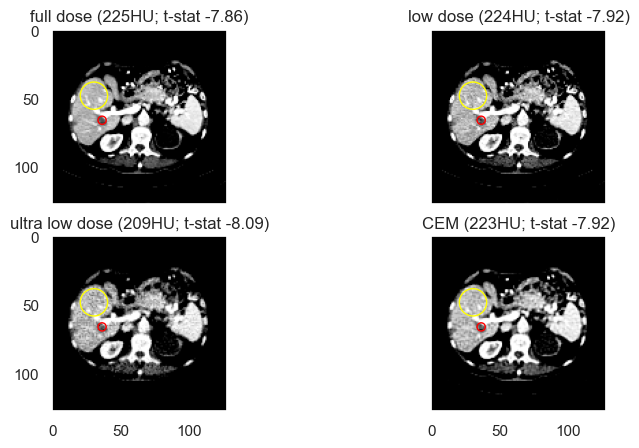
\includegraphics[width=.9\linewidth]{./.ob-jupyter/e740404a2befda3f577afd66c37d89a71ea77324.png}
\end{center}


\begin{minted}[,frame=single, linenos, breaklines, tabsize=2]{python}
import utils
import h5py
from pathlib import Path

ww = 350
wl = 50

plt.clf()
plt.imshow(images[0], cmap=plt.cm.Greys_r)
plt.grid(None)
plt.savefig('cem_sample1.png')


with h5py.File(f'{Path.home()}/Documents/bayesian-inversion/cem_samples.hdf5', 'r') as hf:
    images = [utils.window_image(img * ww - wl, ww, wl) for img in hf['samples'][:9]]
plt.clf()
utils.show_img_grid(images)

\end{minted}

\begin{verbatim}
<Figure size 640x480 with 0 Axes>
\end{verbatim}

\begin{center}
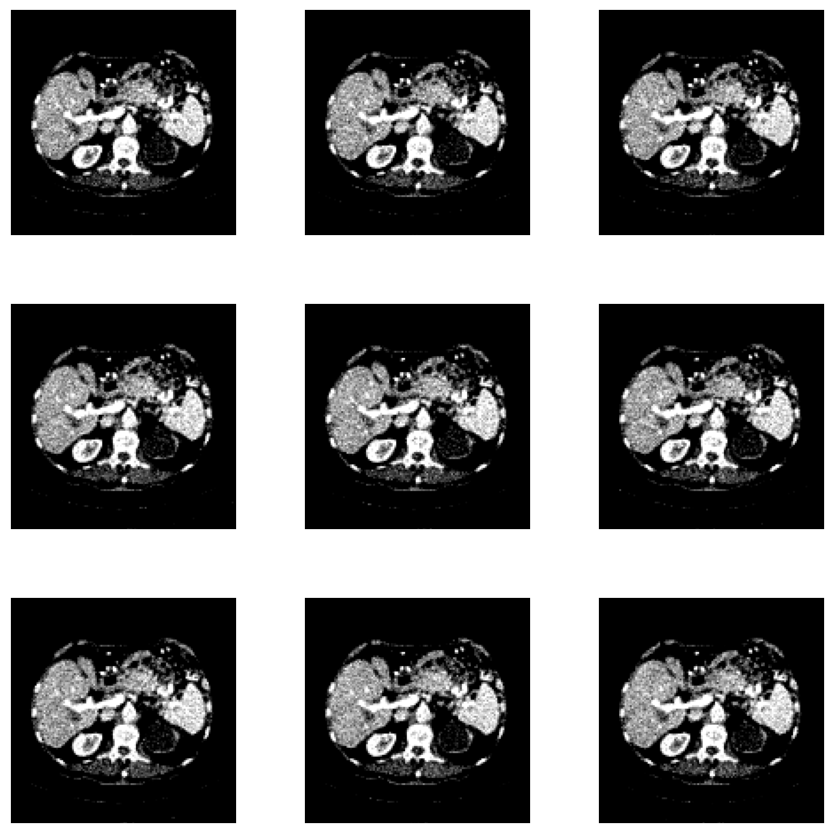
\includegraphics[width=.9\linewidth]{./.ob-jupyter/b5966c204c66decb8494e2253ff0c5c519a92527.png}
\end{center}

\section{Reads}
\label{sec:orgd50265e}
\begin{itemize}
\item Quick summary on CR reconstruciton and Helical CT \url{http://xrayphysics.com/ctsim.html}
\item Example to perform simple image reconstruction using scikit-image \url{https://scikit-image.org/docs/stable/auto\_examples/transform/plot\_radon\_transform.html}
\item Python code to reconstruct image from helical scans? \url{https://github.com/dzwiedzn7/filtered-back-projection/blob/master/tompy.py}
\item Python code to simulate thick slice images from Helical scans \url{https://github.com/Feanor007/Thin2Thick}
\item Python library for Tomography \url{https://pypi.org/project/algotom/}
\item C code for Model-Based Iterative Reconstruciton code for Multi-Slice Helical Geometry \url{https://github.com/cabouman/OpenMBIR-Index/blob/master/README.md}
\item General summary for 3D image reconstruction \url{https://humanhealth.iaea.org/HHW/MedicalPhysics/NuclearMedicine/ImageAnalysis/3Dimagereconstruction/index.html}
\item Pyro-NN: Generalized Python code for image reconstruction using deep learning implemented in Tensorflow code \url{https://www.ncbi.nlm.nih.gov/pmc/articles/PMC6899669/}
\item TomoPy: python library for tomographic data analysis \url{https://www.ncbi.nlm.nih.gov/pmc/articles/PMC4181643/}
\item Powerpoint presentation on CT image reconstruction \url{http://www.sci.utah.edu/\~shireen/pdfs/tutorials/Elhabian\_CT09.pdf}
\item Astra toolbox: python matlab library for 2D/3D tomography \url{https://github.com/astra-toolbox/astra-toolbox}
\item Operator Discretization Library (ODL): used by authors of the paper and has example Python code to reconstruct image from Helical scans \url{https://github.com/odlgroup/odl/tree/master/examples/tomo}
\item matlab code for simple low-dose CT samples simulation \url{https://github.com/smuzd/LD-CT-simulation/tree/master}
\item matlab code for 2nd winner from 2016 Mayo Grand Challenge \url{https://github.com/jongcye/deeplearningLDCT/tree/master}
\item Jupyter code to add white noise to CT scans. May have code to reconstruct images from Helical scans? \url{https://github.com/ayaanzhaque/Noise2Quality}
\item Alternative CT training data? \url{https://www.kaggle.com/c/data-science-bowl-2017/overview}
\item Alternative CT training data from piglets? \url{https://link.springer.com/article/10.1007/s10278-018-0056-0}
\end{itemize}
\section{References}
\label{sec:org75d9450}
\noindent
Adler, Jonas and Öktem, Ozan (2018). \emph{Deep {{Bayesian Inversion}}}.

\noindent
Elhamiasl, Masoud and Nuyts, Johan (2020). \emph{Low-Dose x-Ray {{CT}} Simulation from an Available Higher-Dose Scan}, IOP Publishing.

\noindent
McCollough, Cynthia H. and Bartley, Adam C. and Carter, Rickey E. and Chen, Baiyu and Drees, Tammy A. and Edwards, Phillip and Holmes, David R. and Huang, Alice E. and Khan, Farhana and Leng, Shuai and McMillan, Kyle L. and Michalak, Gregory J. and Nunez, Kristina M. and Yu, Lifeng and Fletcher, Joel G. (2017). \emph{Low-Dose {{CT}} for the Detection and Classification of Metastatic Liver Lesions: {{Results}} of the 2016 {{Low Dose CT Grand Challenge}}}.

\noindent
Moen, Taylor R. and Chen, Baiyu and Holmes III, David R. and Duan, Xinhui and Yu, Zhicong and Yu, Lifeng and Leng, Shuai and Fletcher, Joel G. and McCollough, Cynthia H. (2021). \emph{Low-Dose {{CT}} Image and Projection Dataset}.

\noindent
Yi, Xin and Babyn, Paul (2018). \emph{Sharpness-Aware {{Low}} Dose {{CT}} Denoising Using Conditional Generative Adversarial Network}.
\end{document}